\documentclass[conference]{IEEEtran}

% -------- Packages --------
\usepackage{amsmath, amssymb, graphicx, cite, hyperref}
\usepackage{tikz}
\usetikzlibrary{calc,arrows.meta,positioning,fit,shapes.geometric}
\usepackage{pgfplots}
\pgfplotsset{compat=1.18}
\usepackage{siunitx}

% ---------- Title ----------
\title{SkyEdge: Secure High-Altitude Drone Platform Integrating $H_\infty$ Control, Domestic Devices, and Advanced Mechanical Design}

% ---------- Author ----------
\author{
\IEEEauthorblockN{Shinichi Samizo}
\IEEEauthorblockA{Independent Semiconductor Researcher \\
Project Design Hub, Samizo-AITL \\
\textit{Email:} \href{mailto:shin3t72@gmail.com}{shin3t72@gmail.com} \\
\textit{GitHub:} \href{https://github.com/Samizo-AITL}{Samizo-AITL}}
}

\begin{document}
\maketitle

% ---------- Abstract ----------
\begin{abstract}
This paper presents the foundational design of \emph{SkyEdge}, 
a secure high-altitude unmanned aerial vehicle (UAV) platform that 
integrates $H_\infty$ control, domestic devices, and a variable-pitch 
mechanical structure. The proposed framework provides robust disturbance 
rejection, secure hardware implementation, and reliable flight capability 
up to 10{,}000 m altitude. We describe the control architecture, device 
integration, and mechanical design, and we outline evaluation plans 
toward a proof-of-concept prototype.
\end{abstract}

% ---------- Keywords ----------
\begin{IEEEkeywords}
UAV, robust control, $H_\infty$, variable-pitch rotor, secure systems, high-altitude flight
\end{IEEEkeywords}

% ---------- Sections ----------
\section{Introduction}
Unmanned aerial vehicles (UAVs) are increasingly important in defense, 
disaster response, and environmental monitoring. However, most commercial 
systems are limited to altitudes below 3{,}000 m, and many rely on 
foreign-made devices with security concerns. This paper aims to establish 
a domestic, secure UAV platform capable of robust operation in 
high-altitude environments.

\section{Related Work}
Control approaches such as PID, adaptive control, and sliding-mode 
control have been applied to UAVs, but robust performance under strong 
disturbances remains challenging. $H_\infty$ control has potential for 
disturbance rejection. Existing high-altitude UAV programs (NASA Helios, 
JAXA HAPS) demonstrate feasibility but rely on specialized designs. 
Security aspects and domestic device integration remain underexplored.

\section{System Architecture}
The proposed architecture integrates three layers:
\begin{itemize}
    \item \textbf{$H_\infty$ Control:} ensures robustness against gusts 
    up to 20--30 m/s.
    \item \textbf{FSM:} manages mode transitions (normal, high-altitude, 
    comm-loss, emergency return).
    \item \textbf{LLM:} assists adaptive redesign of control policies in 
    unforeseen conditions (simulation environment).
\end{itemize}

% ===== Fig.1 (two-column, system architecture) =====
\begin{figure*}[t]
\centering
\resizebox{\textwidth}{!}{%
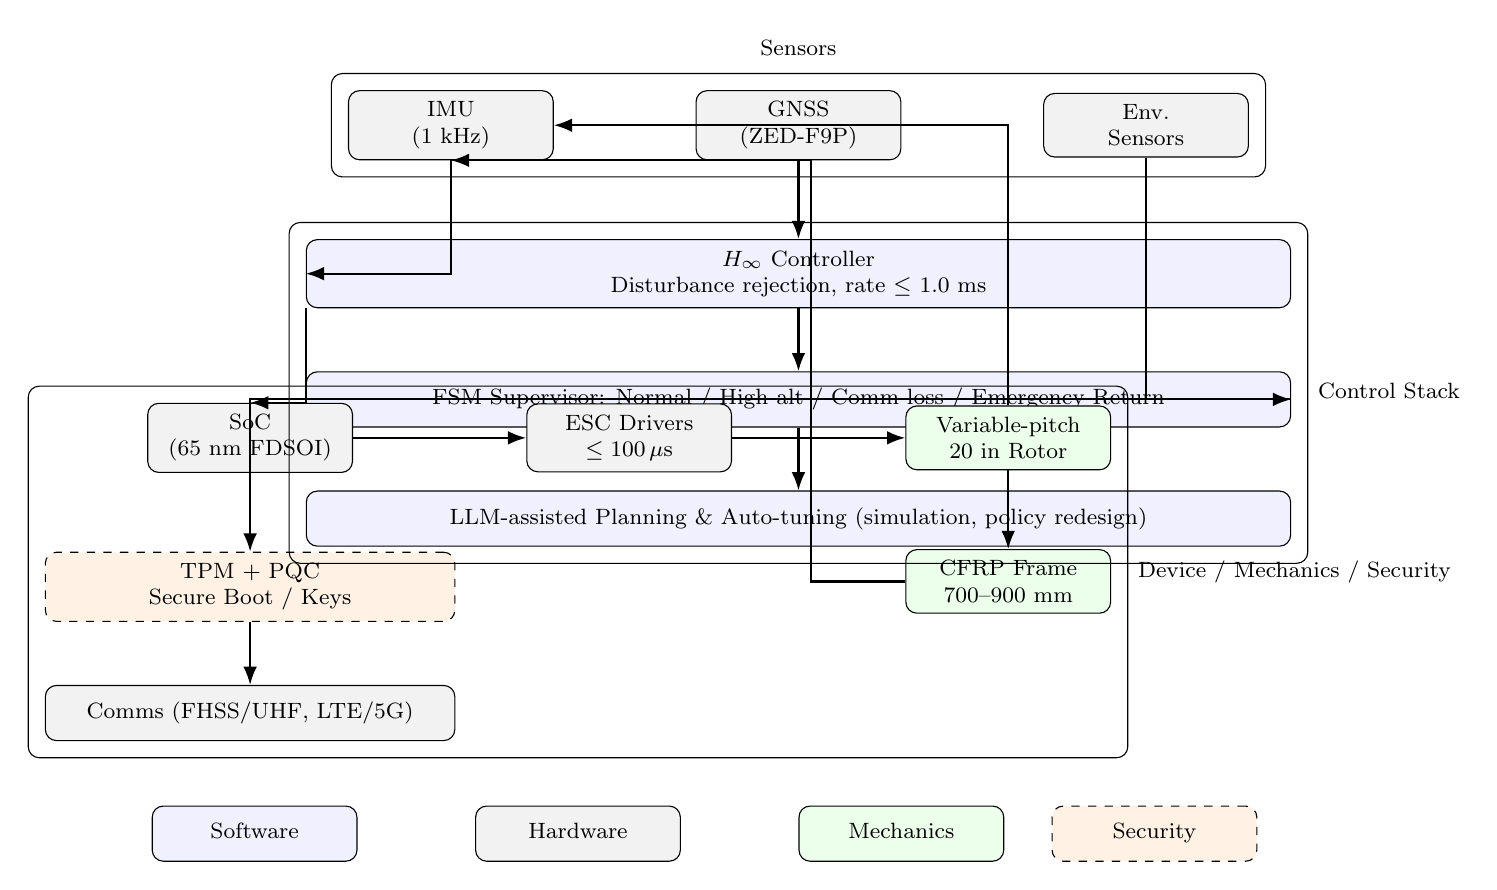
\begin{tikzpicture}[
    font=\footnotesize,
    node distance=8mm and 12mm,
    box/.style={draw, rounded corners, align=center, inner sep=4pt, minimum width=2.6cm, minimum height=7mm},
    hw/.style={box, fill=gray!10},
    sw/.style={box, fill=blue!6},
    mech/.style={box, fill=green!8},
    sec/.style={box, fill=orange!10, dashed},
    arrow/.style={-Latex, thick},
    grp/.style={draw, rounded corners, inner sep=6pt}
]

% Sensors
\node[hw] (imu) {IMU\\(1 kHz)};
\node[hw, right=18mm of imu] (gps) {GNSS\\(ZED-F9P)};
\node[hw, right=18mm of gps] (env) {Env.\\Sensors};

% H-infinity control
\node[sw, below=10mm of gps, minimum width=12.5cm] (hinf) {$H_\infty$ Controller\\
Disturbance rejection, rate $\leq$ 1.0 ms};

% FSM / LLM
\node[sw, below=8mm of hinf, minimum width=12.5cm] (fsm) {FSM Supervisor: Normal / High-alt / Comm-loss / Emergency Return};
\node[sw, below=8mm of fsm, minimum width=12.5cm] (llm) {LLM-assisted Planning \& Auto-tuning (simulation, policy redesign)};

% Hardware row
\node[hw, below left=12mm and -6mm of hinf] (soc) {SoC\\(65 nm FDSOI)};
\node[hw, right=22mm of soc] (esc) {ESC Drivers\\$\leq 100\,\mu$s};
\node[mech, right=22mm of esc] (vp) {Variable-pitch\\20 in Rotor};

% Mechanics / Security / Comms
\node[mech, below=10mm of vp] (frame) {CFRP Frame\\700--900 mm};
\node[sec, below=10mm of soc, minimum width=5.2cm] (secblk) {TPM + PQC\\Secure Boot / Keys};
\node[hw, below=8mm of secblk, minimum width=5.2cm] (comms) {Comms (FHSS/UHF, LTE/5G)};

% Groups
\node[grp, fit=(imu)(gps)(env), label=above:{\strut Sensors}] (gSensors) {};
\node[grp, fit=(hinf)(fsm)(llm), label=right:{\strut Control Stack}] (gCtrl) {};
\node[grp, fit=(soc)(esc)(vp)(frame)(secblk)(comms),
      label=right:{\strut Device / Mechanics / Security}] (gHW) {};

% Connections
\draw[arrow] (imu.south) |- (hinf.west);
\draw[arrow] (gps.south) -- (hinf.north);
\draw[arrow] (env.south) |- (fsm.east);

\draw[arrow] (hinf.south) -- (fsm.north);
\draw[arrow] (fsm.south) -- (llm.north);

\draw[arrow] (hinf.south west) |- (soc.north);
\draw[arrow] (soc.east) -- (esc.west);
\draw[arrow] (esc.east) -- (vp.west);
\draw[arrow] (vp.south) -- (frame.north);

\draw[arrow] (fsm.east) -| (secblk.north);
\draw[arrow] (secblk.south) -- (comms.north);

% Feedback
\draw[arrow] (frame.west) -| ++(-12mm,0) |- (imu.south);
\draw[arrow] (vp.north) |- (imu.east);

% Legend
\path (gHW.south) ++(0,-6mm) coordinate (leg);
\node[box, fill=blue!6,  anchor=north east] (lg1) at ($(leg)+(-28mm,0)$) {\strut Software};
\node[box, fill=gray!10, anchor=north]      (lg2) at (leg)               {\strut Hardware};
\node[box, fill=green!8, anchor=north west] (lg3) at ($(leg)+(28mm,0)$)   {\strut Mechanics};
\node[box, fill=orange!10, dashed, anchor=north west] (lg4)
      at ($(lg3.north east)+(6mm,0)$) {\strut Security};

\end{tikzpicture}%
}
\caption{SkyEdge system architecture (two-column figure). The three-layer control stack ($H_\infty$, FSM, LLM) integrates with sensors, a secure device stack (SoC, TPM/PQC, comms), and variable-pitch mechanical design.}
\label{fig:sysarch}
\end{figure*}

% ===== Fig.2 (gust step response, Hinf vs PID) =====
\begin{figure*}[t]
\centering
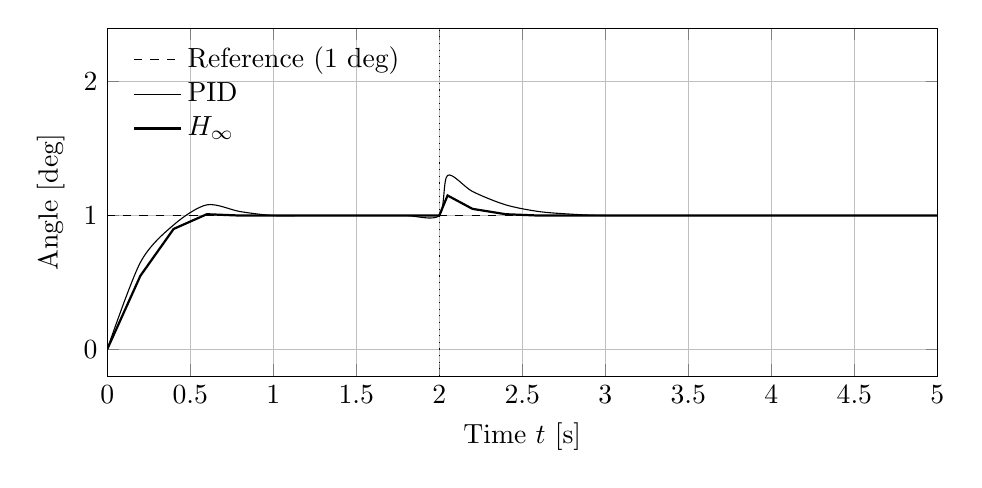
\begin{tikzpicture}
\begin{axis}[
    width=\textwidth, height=6.0cm,
    xlabel={Time $t$ [s]}, ylabel={Angle [deg]},
    xmin=0, xmax=5, ymin=-0.2, ymax=2.4,
    grid=both, legend cell align=left,
    legend style={at={(0.02,0.98)},anchor=north west,draw=none,fill=none},
    tick label style={/pgf/number format/fixed},
]
\addplot[dashed] coordinates {(0,0) (0.001,0) (0.001,1) (5,1)};
\addlegendentry{Reference (1 deg)}
\addplot[smooth] coordinates {
(0,0) (0.2,0.65) (0.4,0.93) (0.6,1.08) (0.8,1.03) (1.0,1.00)
(1.2,1.00) (1.4,1.00) (1.6,1.00) (1.8,1.00)
(2.0,1.00) (2.05,1.30) (2.2,1.18) (2.4,1.08) (2.6,1.03) (2.8,1.01)
(3.0,1.00) (3.4,1.00) (3.8,1.00) (4.2,1.00) (4.6,1.00) (5.0,1.00)
};
\addlegendentry{PID}
\addplot[thick] coordinates {
(0,0) (0.2,0.55) (0.4,0.90) (0.6,1.01) (0.8,1.00) (1.0,1.00)
(1.2,1.00) (1.4,1.00) (1.6,1.00) (1.8,1.00)
(2.0,1.00) (2.05,1.15) (2.2,1.05) (2.4,1.01) (2.6,1.00)
(2.8,1.00) (3.0,1.00) (3.5,1.00) (4.0,1.00) (4.5,1.00) (5.0,1.00)
};
\addlegendentry{$H_\infty$}
\draw[dotted] (axis cs:2,-0.2) -- (axis cs:2,2.4);
\node[anchor=south east] at (axis cs:2,2.35) {Gust $+15\%$ at $t{=}2$ s};
\end{axis}
\end{tikzpicture}
\caption{Step tracking with a sudden gust. The $H_\infty$ controller yields smaller overshoot and faster recovery than PID when a $+15\%$ gust hits at $t=2$ s.}
\label{fig:resp_gust}
\end{figure*}

% ===== Fig.3 (thrust margin vs altitude) =====
\begin{figure*}[t]
\centering
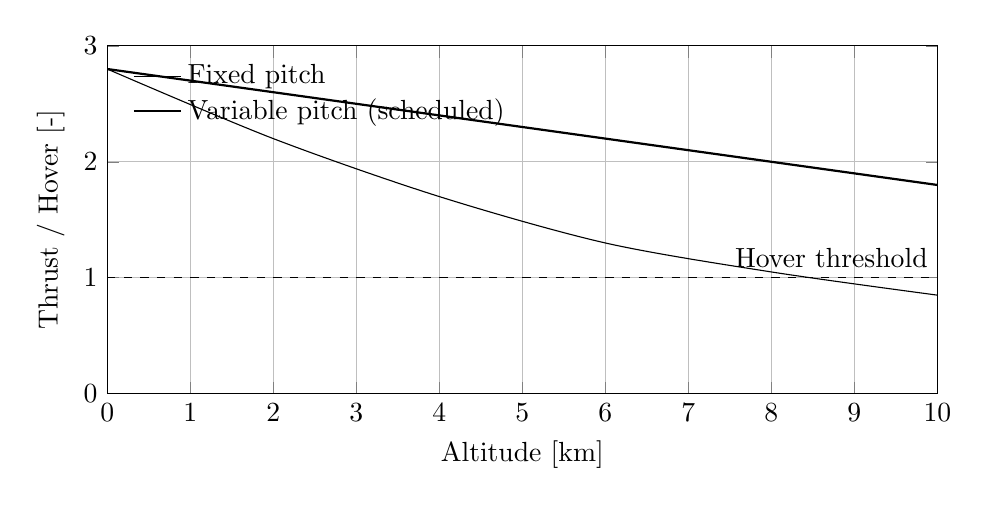
\begin{tikzpicture}
\begin{axis}[
    width=\textwidth, height=6.0cm,
    xlabel={Altitude [km]}, ylabel={Thrust / Hover [-]},
    xmin=0, xmax=10, ymin=0, ymax=3.0,
    grid=both, legend cell align=left,
    legend style={at={(0.02,0.98)},anchor=north west,draw=none,fill=none},
]
\addplot[smooth] coordinates {
(0,2.8) (2,2.2) (4,1.7) (6,1.3) (8,1.05) (10,0.85)
};
\addlegendentry{Fixed pitch}
\addplot[thick,smooth] coordinates {
(0,2.8) (2,2.6) (4,2.4) (6,2.2) (8,2.0) (10,1.8)
};
\addlegendentry{Variable pitch (scheduled)}
\addplot[dashed,domain=0:10] {1};
\node[anchor=south east] at (axis cs:10,1) {Hover threshold};
\end{axis}
\end{tikzpicture}
\caption{Thrust margin vs. altitude. Pitch scheduling maintains a thrust/hover ratio above 1 up to 10 km, while a fixed-pitch rotor loses margin.}
\label{fig:thrust_altitude}
\end{figure*}

% ===== Fig.4 (servo torque vs pitch angle) =====
\begin{figure*}[t]
\centering
\begin{tikzpicture}
\begin{axis}[
    width=\textwidth, height=6.0cm,
    xlabel={Pitch angle [$^\circ$]}, ylabel={Required servo torque [N$\cdot$m]},
    xmin=0, xmax=20, ymin=0, ymax=1.6,
    grid=both, legend style={at={(0.02,0.98)},anchor=north west,draw=none,fill=none},
]
\addplot[thick,domain=0:20,samples=200] {0.02 + 0.03*x + 0.0015*x*x};
\addlegendentry{Required torque (model)}
\addplot[only marks,mark=*] coordinates {(12,0.62)};
\node[anchor=south west] at (axis cs:12,0.62) {Design point};
\addplot[name path=a,domain=0:20,samples=200] {2*(0.02 + 0.03*x + 0.0015*x*x)};
\addplot[name path=b,domain=0:20,samples=200] {3*(0.02 + 0.03*x + 0.0015*x*x)};
\addplot[fill=black!10,draw=none] fill between[of=a and b];
\node[anchor=south east] at (axis cs:19.8,1.5) {Safety band ($\times 2\sim 3$)};
\end{axis}
\end{tikzpicture}
\caption{Servo torque vs. pitch angle for the variable-pitch mechanism. The design point around \SI{0.62}{N.m} leaves a safety margin of $\times 2\sim 3$.}
\label{fig:servo_torque}
\end{figure*}

% ===== Fig.5 (frequency-domain intuition for Hinf) =====
\begin{figure*}[t]
\centering
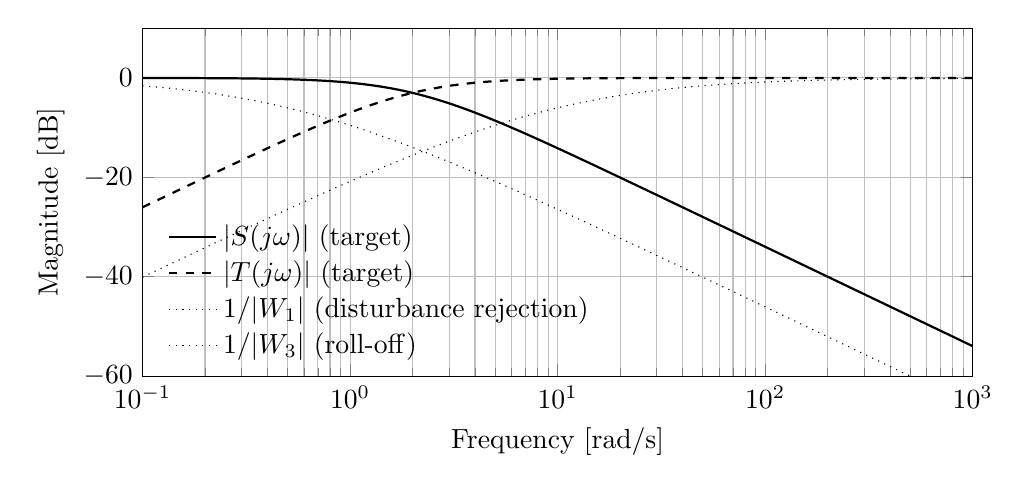
\begin{tikzpicture}
\begin{semilogxaxis}[
    width=\textwidth, height=6.0cm,
    xlabel={Frequency [rad/s]}, ylabel={Magnitude [dB]},
    xmin=1e-1, xmax=1e3, ymin=-60, ymax=10,
    grid=both, legend cell align=left,
    legend style={at={(0.02,0.02)},anchor=south west,draw=none,fill=none},
]
\addplot[thick,domain=1e-1:1e3,samples=400] {-20*log10(sqrt(1 + (x/2)^2))};
\addlegendentry{$|S(j\omega)|$ (target)}
\addplot[thick,dashed,domain=1e-1:1e3,samples=400] {-20*log10(sqrt(1 + (2/x)^2))};
\addlegendentry{$|T(j\omega)|$ (target)}
\addplot[dotted,domain=1e-1:1e3,samples=400] {-20*log10(1 + x/0.5)};
\addlegendentry{$1/|W_1|$ (disturbance rejection)}
\addplot[dotted,domain=1e-1:1e3,samples=400] {-20*log10(1 + 10/x)};
\addlegendentry{$1/|W_3|$ (roll-off)}
\end{semilogxaxis}
\end{tikzpicture}
\caption{Frequency-domain intuition for $H_\infty$ design: low $|S|$ in low–mid frequency (disturbance rejection) and low $|T|$ in high frequency (noise/roll-off).}
\label{fig:freq_ST}
\end{figure*}

\section{Device Integration}
The device layer includes a domestic SoC (65 nm FDSOI), LDMOS motor 
drivers, high-rate IMU (1 kHz), and secure modules (TPM + PQC). 
Control cycle is maintained at $\leq 1.0$ ms with ESC response $\leq 100 
\, \mu$s. Estimated BOM cost is 596{,}700 JPY per unit (with reduction in 
mass production).

\section{Mechanical Design}
The UAV has a 700--900 mm frame, CFRP structure, and a variable-pitch 
20-inch rotor system. At take-off weight 6.38 kg, the thrust-to-weight 
ratio is $\approx 2.82$. Variable pitch enables adaptation from sea 
level to 10{,}000 m (RPM from $\approx 8{,}339$ to $14{,}353$). Servo torque 
requirement is 0.62 N$\cdot$m with safety factor of 2--3.

\section{Evaluation Plan}
Planned evaluations include wind-tunnel testing, low-temperature chamber 
tests, redundancy verification, and communication robustness under 
jamming scenarios. A proof-of-concept schedule has been drafted for 
2025--2026.

\section{Conclusion}
We presented the SkyEdge architecture integrating $H_\infty$ control, 
domestic devices, and mechanical design for secure high-altitude UAVs. 
The proposed system addresses robustness, security, and reliability at 
10{,}000 m operation. Future work includes prototype development and 
extension to underwater vehicles (\emph{SeaEdge}), toward a unified 
autonomous platform for defense, disaster response, GX, and education.

% ---------- References ----------
\bibliographystyle{IEEEtran}
\bibliography{refs}

\end{document}
